% LaTeX Template for Project Report, Version 1.0

% Created by: Ernest Mwebaze
%Revised by: Azamuke Denish


\documentclass[12pt, a4paper]{report}
\usepackage[pdftex]{graphicx} %for embedding images
\usepackage{url} %for proper url entries
% \usepackage[bookmarks, colorlinks=false, pdfborder={0 0 0}, pdftitle={<pdf title here>}, pdfauthor={<author's name here>}, pdfsubject={<subject here>}, pdfkeywords={<keywords here>}]{hyperref} %for creating links in the pdf version and other additional pdf attributes, no effect on the printed document
%\usepackage[final]{pdfpages} %for embedding another pdf, remove if not required

\begin{document}
\renewcommand\bibname{References} %Renames "Bibliography" to "References" on ref page

\pagenumbering{roman} %numbering before main content starts
%Include first stuff: title, acknowledgement, dedication, tables, etc
\begin{titlepage}

\begin{center}


\includegraphics[width=1\textwidth]{img/maklogo}\\%\\[0.1in]
\vspace{3em}%
% Title
\Large \textbf {[Your project title]}\\%\\[0.5in]
\vspace{1em}%
\normalsize by \\%
\vspace{1em}
\textup{\small {\bf [Your group name]}\\}
 \vspace{1em}%
{\bf Department of Computer Science \\ School of Computing \& Informatics Technology}\\[0.5in]

\emph{A Project Report Submitted to the \\School of Computing and Informatics Technology
for the Study Leading to\\ a Project Report in Partial Fulfilment of the
requirements for the\\ Award of the Degree of Bachelor of Science in \\Computer Science
of Makerere University}

       % \small \emph{Submitted in partial fulfillment of\\
       %  the requirements for the award of the degree of}
        \vspace{1in}

       

% Submitted by
\normalsize {\bf Supervisor:} \\

[Supervisor's name]\\
\vspace{1em}
Department of Computer Science\\
School of Computing \& Informatics Technology \\
% \vspace{1em}
\url{supervisor@cis.mak.ac.ug} Tel: $+256$ Fax: $+256$
% \begin{table}[h]
% \centering
% \begin{tabular}{lr}\hline \\
% Roll No & Names of Students \\ \\ \hline
% \\
% <Roll no here> & <Name here> \\
% <Roll no here> & <Name here> \\ 
% <Roll no here> & <Name here> \\ \\ \hline 
% \end{tabular}
% \end{table}

% \vspace{.1in}
% \date{}\\
% {\textbf{<Guide's name here>}}\\[0.2in]

\vfill

% Bottom of the page
% \includegraphics[width=0.18\textwidth]{./nitc-logo}\\[0.1in]
% \Large{Department of Computer Science and Engineering}\\
% \normalsize
% \textsc{National Institute of Technology Calicut}\\
% Calicut, Kerala, India -- 673 601 \\
% \vspace{0.2cm}
April, 2019

\end{center}

\end{titlepage}

\cleardoublepage
\addcontentsline{toc}{chapter}{Declaration}
\chapter*{Declaration}
We Group [Group Name] do hereby declare that this Project Report is original and has not been published and/or submitted for any other degree award to any other University before.


\begin{table}[!ht]
\centering
\resizebox{\textwidth}{!}{%
\begin{tabular}{|l|l|l|l|}
\hline
\textbf{\#} & \textbf{Names}  & \textbf{Registration Number} & \textbf{Signature} \\ \hline
1           & Fresh Kid    & 16/U/2345/PS                 &                    \\ \hline
2           & Bryan White & 16/T/8702/EVE                &                    \\ \hline
3           & Joseph Kony   & 16/U/9867/PS                 &                    \\ \hline
4           & Sheebah Karungi  & 16/U/324                     &                    \\ \hline
\end{tabular}%
}
\end{table}
\vspace{1.0in}
\noindent
Date: \\
-----------------------------------------------------------------------------------
\newpage

\cleardoublepage
\addcontentsline{toc}{chapter}{Approval}
\chapter*{Approval}
This Project Report has been submitted for examination with the approval of the following supervisor.

\vspace{1.0em}
\noindent
Signed: \\
-----------------------------------------------------------------------------------\\
Date: \\
-----------------------------------------------------------------------------------\\

\vspace{2.0em}

\noindent
[Supervisor's name] \\
BSc. CS, MSc. CS,\\
School of Computing \& IT\\
College of Computing \& IT\\
Makerere University\\
\emph{supervisor@cis.mak.ac.ug}
\newpage

\cleardoublepage
\addcontentsline{toc}{chapter}{Dedication}
\chapter*{Dedication}
We dedicate this report to the Almighty God without whom we can do nothing.
We further dedicate it to our parents and guardians for their unceasing and selfless support throughout our stay in this university.
\newpage

\cleardoublepage
\addcontentsline{toc}{chapter}{Acknowledgement}
\chapter*{Acknowledgement}
We are deeply indebted to our project supervisor [Supervisor's name] whose unlimited steadfast support and inspirations have made this project a great success. In a very special way, we thank him for every support he has rendered unto us to see that we succeed in this challenging study.

Special thanks go to our friends and families who have contained the hectic moments and stress we have been through during the course of the research project.

We thank the school for giving us the grand opportunity to work as a team which has indeed promoted our team work spirit and communication skills. We also thank the individual group members for the good team spirit and solidarity.

\newpage

% \tableofcontents
% \input{./certificate.tex}
% %Two resources useful for abstract writing.
% Guidance of how to write an abstract/summary provided by Nature: https://cbs.umn.edu/sites/cbs.umn.edu/files/public/downloads/Annotated_Nature_abstract.pdf %https://writingcenter.gmu.edu/guides/writing-an-abstract
\chapter*{\center \Large  Abstract}
%%%%%%%%%%%%%%%%%%%%%%%%%%%%%%%%%%%%%%
% Replace all text with your text
%%%%%%%%%%%%%%%%%%%%%%%%%%%%%%%%%%%

This is an undergraduate project report template and instruction on how to write a report. It also has some useful examples to use \LaTeX. Do read this template carefully. The number of chapters and their titles may vary depending on the type of project and personal preference. Section titles in this template are illustrative should be updated accordingly. For example, sections named ``A section...'' and ``Example of ...'' should be updated. The number of sections in each chapter may also vary. This template may or may not suit your project. Discuss the structure of your report with your supervisor.

%%%
~\\[1cm]%REMOVE THIS
\noindent\textbf{Guidance on abstract writing:} An abstract is a summary of a report in a single paragraph up to a maximum of 250 words. An abstract should be self-contained, and it should not refer to sections, figures, tables, equations, or references. An abstract typically consists of sentences describing the following four parts: (1) introduction (background and purpose of the project), (2) methods, (3) results and analysis, and (4) conclusions. The distribution of these four parts of the abstract should reflect the relative proportion of these parts in the report itself. An abstract starts with a few sentences describing the project's general field, comprehensive background and context, the main purpose of the project; and the problem statement. A few sentences describe the methods, experiments, and implementation of the project. A few sentences describe the main results achieved and their significance. The final part of the abstract describes the conclusions and the implications of the results to the relevant field.


%%%%%%%%%%%%%%%%%%%%%%%%%%%%%%%%%%%%%%%%%%%%%%%%%%%%%%%%%%%%%%%%%%%%%%%%%s
~\\[1cm]
\noindent % Provide your key words
\textbf{Keywords:} a maximum of five keywords/keyphrase separated by commas

\vfill
\noindent
\textbf{Report's total word count:} we expect a maximum of 20,000 words (excluding reference and appendices) and about 50 - 60 pages. [A good project report can also be written in approximately 10,000 words.]


\tableofcontents
\listoffigures
\listoftables

\newpage
\pagenumbering{arabic} %reset numbering to normal for the main content

% \input{./prob-definition.tex} %objective changed to problem definition
\chapter{Introduction}
\label{ch:into} % This how you label a chapter and the key (e.g., ch:into) will be used to refer this chapter ``Introduction'' later in the report. 
% the key ``ch:into'' can be used with command \ref{ch:intor} to refere this Chapter.

\textbf{Guidance on introduction chapter writing:} Introductions are written in the following parts:
\begin{itemize}
    \item A brief  description of the investigated problem.
    \item A summary of the scope and context of the project, i.e., what is the background of the topic/problem/application/system/algorithm/experiment/research question/hypothesis/etc. under investigation/implementation/development [whichever is applicable to your project].
    \item The aims and objectives of the project.
    \item A description of the problem and the methodological approach adopted to solve the problem.
    \item A summary of the most significant outcomes and their interpretations.
    \item Organization of the report. 
\end{itemize}


Consult \textbf{your supervisor} to check the content of the introduction chapter. In this template, we only offer basic sections of an introduction chapter. It may  not be complete and comprehensive. Writing a report is a subjective matter, and a report's style and structure depend on the ``type of project'' as well as an individual's preference. This template suits the following project paradigms:
\begin{enumerate}
    \item software engineering and software/web application development;
    \item algorithm implementation, analysis and/or application;  
    \item science lab (experiment); and
    \item pure theoretical development (not mention extensively).
\end{enumerate}

Use only a single \textbf{font} for the body text. We recommend using a clean and electronic document friendly font like \textbf{Arial} or \textbf{Calibri} for MS-word (If you create a report in MS word). If you use this template, DO NOT ALTER the template's default font ``amsfont default computer modern''. The default \LaTeX~font ``computer modern'' is also acceptable. 

The recommended body text \textbf{font size} is minimum \textbf{11pt} and minimum one-half line spacing. The recommended figure/table caption font size is minimum 10pt. The footnote\footnote{Example footnote: footnotes are useful for adding external sources such as links as well as extra information on a topic or word or sentence. Use command \textbackslash footnote\{...\} next to a word to generate a footnote in \LaTeX.} font size is minimum 8pt. DO NOT ALTER the font setting of this template.   

%%%%%%%%%%%%%%%%%%%%%%%%%%%%%%%%%%%%%%%%%%%%%%%%%%%%%%%%%%%%%%%%%%%%%%%%%%%%%%%%%%%
\section{Background}
\label{sec:into_back}
Describe to a reader the context of your project. That is, what is your project and what its motivation. Briefly explain the major theories, applications, and/or products/systems/algorithms whichever is relevant to your project.

\textbf{Cautions:} Do not say you choose this project because of your interest, or your supervisor proposed/suggested this project, or you were assigned this project as your final year project. This all may be true, but it is not meant to be written here.

%%%%%%%%%%%%%%%%%%%%%%%%%%%%%%%%%%%%%%%%%%%%%%%%%%%%%%%%%%%%%%%%%%%%%%%%%%%%%%%%%%%
\section{Problem statement}
\label{sec:intro_prob_art}
This section describes the investigated problem in detail. You can also have a separate chapter on ``Problem articulation.''  For some projects, you may have a section like ``Research question(s)'' or ``Research Hypothesis'' instead of a section on ``Problem statement.'

%%%%%%%%%%%%%%%%%%%%%%%%%%%%%%%%%%%%%%%%%%%%%%%%%%%%%%%%%%%%%%%%%%%%%%%%%%%%%%%%%%%
\section{Aims and objectives}
\label{sec:intro_aims_obj}
Describe the ``aims and objectives'' of your project. 

\textbf{Aims:} The aims tell a read what you want/hope to achieve at the end of the project. The  aims define your intent/purpose in general terms.  

\textbf{Objectives:} The objectives are a set of tasks you would perform in order to achieve the defined aims. The objective statements have to be specific and measurable through the results and outcome of the project.



%%%%%%%%%%%%%%%%%%%%%%%%%%%%%%%%%%%%%%%%%%%%%%%%%%%%%%%%%%%%%%%%%%%%%%%%%%%%%%%%%%%
\section{Solution approach}
\label{sec:intro_sol} % label of Org section
Briefly describe the solution approach and the methodology applied in solving the set aims and objectives.

Depending on the project, you may like to alter the ``heading'' of this section. Check with you supervisor. Also, check what subsection or any other section that can be added in or removed from this template.

\subsection{A subsection 1}
\label{sec:intro_some_sub1}
You may or may not need subsections here. Depending on your project's needs, add two or more subsection(s). A section takes at least two subsections. 

\subsection{A subsection 2}
\label{sec:intro_some_sub2}
Depending on your project's needs, add more section(s) and subsection(s).

\subsubsection{A subsection 1 of a subsection}
\label{sec:intro_some_subsub1}
The command \textbackslash subsubsection\{\} creates a paragraph heading in \LaTeX.

\subsubsection{A subsection 2 of a subsection}
\label{sec:intro_some_subsub2}
Write your text here...

%%%%%%%%%%%%%%%%%%%%%%%%%%%%%%%%%%%%%%%%%%%%%%%%%%%%%%%%%%%%%%%%%%%%%%%%%%%%%%%%%%%
\section{Summary of contributions and achievements} %  use this section 
\label{sec:intro_sum_results} % label of summary of results
Describe clearly what you have done/created/achieved and what the major results and their implications are. 


%%%%%%%%%%%%%%%%%%%%%%%%%%%%%%%%%%%%%%%%%%%%%%%%%%%%%%%%%%%%%%%%%%%%%%%%%%%%%%%%%%%
\section{Organization of the report} %  use this section
\label{sec:intro_org} % label of Org section
Describe the outline of the rest of the report here. Let the reader know what to expect ahead in the report. Describe how you have organized your report. 

\textbf{Example: how to refer a chapter, section, subsection}. This report is organised into seven chapters. Chapter~\ref{ch:lit_rev} details the literature review of this project. In Section~\ref{ch:method}...  % and so on.

\textbf{Note:}  Take care of the word like ``Chapter,'' ``Section,'' ``Figure'' etc. before the \LaTeX command \textbackslash ref\{\}. Otherwise, a  sentence will be confusing. For example, In \ref{ch:lit_rev} literature review is described. In this sentence, the word ``Chapter'' is missing. Therefore, a reader would not know whether 2 is for a Chapter or a Section or a Figure.

 %literature survey included in this
\chapter{Literature Review}

\section{Introduction}
The main purpose of this chapter is to present some general consensus on the theoretical support and previous empirical studies on...........


% replace all text with your own text.
% in this template few examples are mention
\chapter{Methodology}
\label{ch:method} % Label for method chapter

We mentioned in Chapter~\ref{ch:into} %[example backward reference to a chapter or section.]
that a project report's structure could follow a particular paradigm. Hence, the organization of a report (effectively the Table of Content of a report) can vary depending on the type of project you are doing. Check which of the given examples suit your project. Alternatively, follow your supervisor's advice.

\section{Examples of the sections of a methodology chapter}
A general report structure is summarised (suggested) in Table~\ref{tab:gen_template}. Table~\ref{tab:gen_template} describes that, in general, a typical report structure has three main parts: (1) front matter, (2) main text, and (3) end matter. %[\textbf{also notice that the preceding sentence is an example of a numbered list in a text body}]. 
The structure of the front matter and end matter will remain the same for all the undergraduate final year project report. However, the main text varies as per the project's needs.
\begin{table}[h!]
    \centering
    \caption{Undergraduate report template structure}
    \label{tab:gen_template}
    \begin{tabular}{llll}     
        \toprule
        \multirow{7}{3cm}{Frontmatter} 
        & & Title Page & \\                  
        & & Abstract &    \\          
        & & Acknowledgements & \\                            
        & & Table of Contents &    \\                                
        & & List of Figures   &    \\                        
        & & List of Tables    &    \\                
        & & List of Abbreviations  &    \\                     
        & &   &    \\                        
        \multirow{7}{3cm}{Main text}
        & Chapter 1 & Introduction   &    \\                         
        & Chapter 2 & Literature Review   &    \\
        & Chapter 3 & Methodology   &    \\
        & Chapter 4 & Results    &    \\
        & Chapter 5 & Discussion and Analysis  &    \\
        & Chapter 6 & Conclusions and Future Work  &    \\        
        & Chapter 7 & Refection  &    \\          
        & &   &    \\                       
        \multirow{2}{3cm}{End matter}
        & & References  &    \\   
        & & Appendices (Optional)  &    \\ 
        & & Index (Optional)  &    \\ 
        \bottomrule
    \end{tabular}
\end{table}

\subsection{Example of a software/Web development main text structure}
\label{subsec:se_chpters}
Notice that the ``methodology'' Chapter of Software/Web development in Table~\ref{tab:soft_eng_temp} takes a standard software engineering paradigm (approach). Alternatively, these suggested sections can be the chapters of their own. Also, notice that ``Chapter 5'' in Table~\ref{tab:soft_eng_temp} is ``Testing and Validation'' which is different from the general report template mentioned in Table~\ref{tab:gen_template}. Check with your supervisor if in doubt.
\begin{table}[h!]
    \centering
    \caption{Example of a software engineering-type report structure}
    \label{tab:soft_eng_temp}
    \begin{tabular}{lll}     
        \toprule                   
        Chapter 1 & Introduction   &    \\        
        Chapter 2 & Literature Review  &    \\                   
        Chapter 3 & Methodology   &    \\
        &               & Requirements specifications   \\
        &               & Analysis   \\
        &               & Design   \\
        &               & Implementations   \\
        Chapter 4 & Testing and Validation  &    \\
        Chapter 5 & Results and Discussion      &    \\
        Chapter 6 & Conclusions and Future Work  &    \\        
        Chapter 7 & Reflection  &    \\                          
        \bottomrule
    \end{tabular}
\end{table}

\subsection{Example of an algorithm analysis main text structure}
Some project might involve the implementation of a state-of-the-art algorithm and its performance analysis and comparison with other algorithms. In that case, the suggestion in Table~\ref{tab:algo_temp} may suit you the best. 
\begin{table}[h!]
    \centering
    \caption{Example of an algorithm analysis type report structure}
    \label{tab:algo_temp}
    \begin{tabular}{lll}     
        \toprule                   
        Chapter 1 & Introduction  &    \\        
        Chapter 2 & Literature Review  &    \\                
        Chapter 3 & Methodology   &    \\
        &               & Algorithms descriptions  \\
        &               & Implementations   \\
        &               & Experiments design   \\
        Chapter 4 & Results       &  \\
        Chapter 5 & Discussion and Analysis  &    \\
        Chapter 6 & Conclusion and Future Work  &    \\        
        Chapter 7 & Reflection  &    \\          
        \bottomrule
    \end{tabular}
\end{table}

\subsection{Example of an application type main text structure}
If you are applying some algorithms/tools/technologies on some problems/datasets/etc., you may use the methodology section prescribed in Table~\ref{tab:app_temp}.  
\begin{table}[h!]
    \centering
    \caption{Example of an application type report structure}
    \label{tab:app_temp}
    \begin{tabular}{lll}     
        \toprule                   
        Chapter 1 & Introduction  &    \\        
        Chapter 2 & Literature Review  &    \\                
        Chapter 3 & Methodology   &    \\
        &               & Problems (tasks) descriptions  \\
        &               & Algorithms/tools/technologies/etc. descriptions  \\        
        &               & Implementations   \\
        &               & Experiments design and setup   \\
        Chapter 4 & Results       &  \\
        Chapter 5 & Discussion and Analysis  &    \\
        Chapter 6 & Conclusion and Future Work  &    \\        
        Chapter 7 & Reflection  &    \\          
        \bottomrule
    \end{tabular}
\end{table}

\subsection{Example of a science lab-type main text structure}
If you are doing a science lab experiment type of project, you may use the  methodology section suggested in Table~\ref{tab:lab_temp}. In this kind of project, you may refer to the ``Methodology'' section as ``Materials and Methods.''
\begin{table}[h!]
    \centering
    \caption{Example of a science lab experiment-type report structure}
    \label{tab:lab_temp}
    \begin{tabular}{lll}     
        \toprule                   
        Chapter 1 & Introduction  &    \\        
        Chapter 2 & Literature Review  &    \\                
        Chapter 3 & Materials and Methods   &    \\
        &               & Problems (tasks) description  \\
        &               & Materials \\        
        &               & Procedures  \\                
        &               & Implementations   \\
        &               & Experiment set-up   \\
        Chapter 4 & Results       &  \\
        Chapter 5 & Discussion and Analysis  &    \\
        Chapter 6 & Conclusion and Future Work  &    \\        
        Chapter 7 & Reflection  &    \\          
        \bottomrule
    \end{tabular}
\end{table}

\section{Example of an Equation in \LaTeX}
Eq.~\ref{eq:eq_example} [note that this is an example of an equation's in-text citation] is an example of an equation in \LaTeX. In Eq.~\eqref{eq:eq_example}, $ s $ is the mean of elements $ x_i \in \mathbf{x} $: 

\begin{equation}
\label{eq:eq_example} % label used to refer the eq in text
s = \frac{1}{N} \sum_{i = 1}^{N} x_i. 
\end{equation}

Have you noticed that all the variables of the equation are defined using the \textbf{in-text} maths command \$.\$, and Eq.~\eqref{eq:eq_example} is treated as a part of the sentence with proper punctuation? Always treat an equation or expression as a part of the sentence. 

\section{Example of a Figure in \LaTeX}
Figure~\ref{fig:chart_a} is an example of a figure in \LaTeX. For more details, check the link:

\href{https://en.wikibooks.org/wiki/LaTeX/Floats,_Figures_and_Captions}{wikibooks.org/wiki/LaTeX/Floats,\_Figures\_and\_Captions}.

\noindent
Keep your artwork (graphics, figures, illustrations) clean and readable. At least 300dpi is a good resolution of a PNG format artwork. However, an SVG format artwork saved as a PDF will produce the best quality graphics. There are numerous tools out there that can produce vector graphics and let you save that as an SVG file and/or as a PDF file. One example of such a tool is the ``Flow algorithm software''. Here is the link for that: \href{http://www.flowgorithm.org/download/}{flowgorithm.org}.
\begin{figure}[ht]
    \centering
    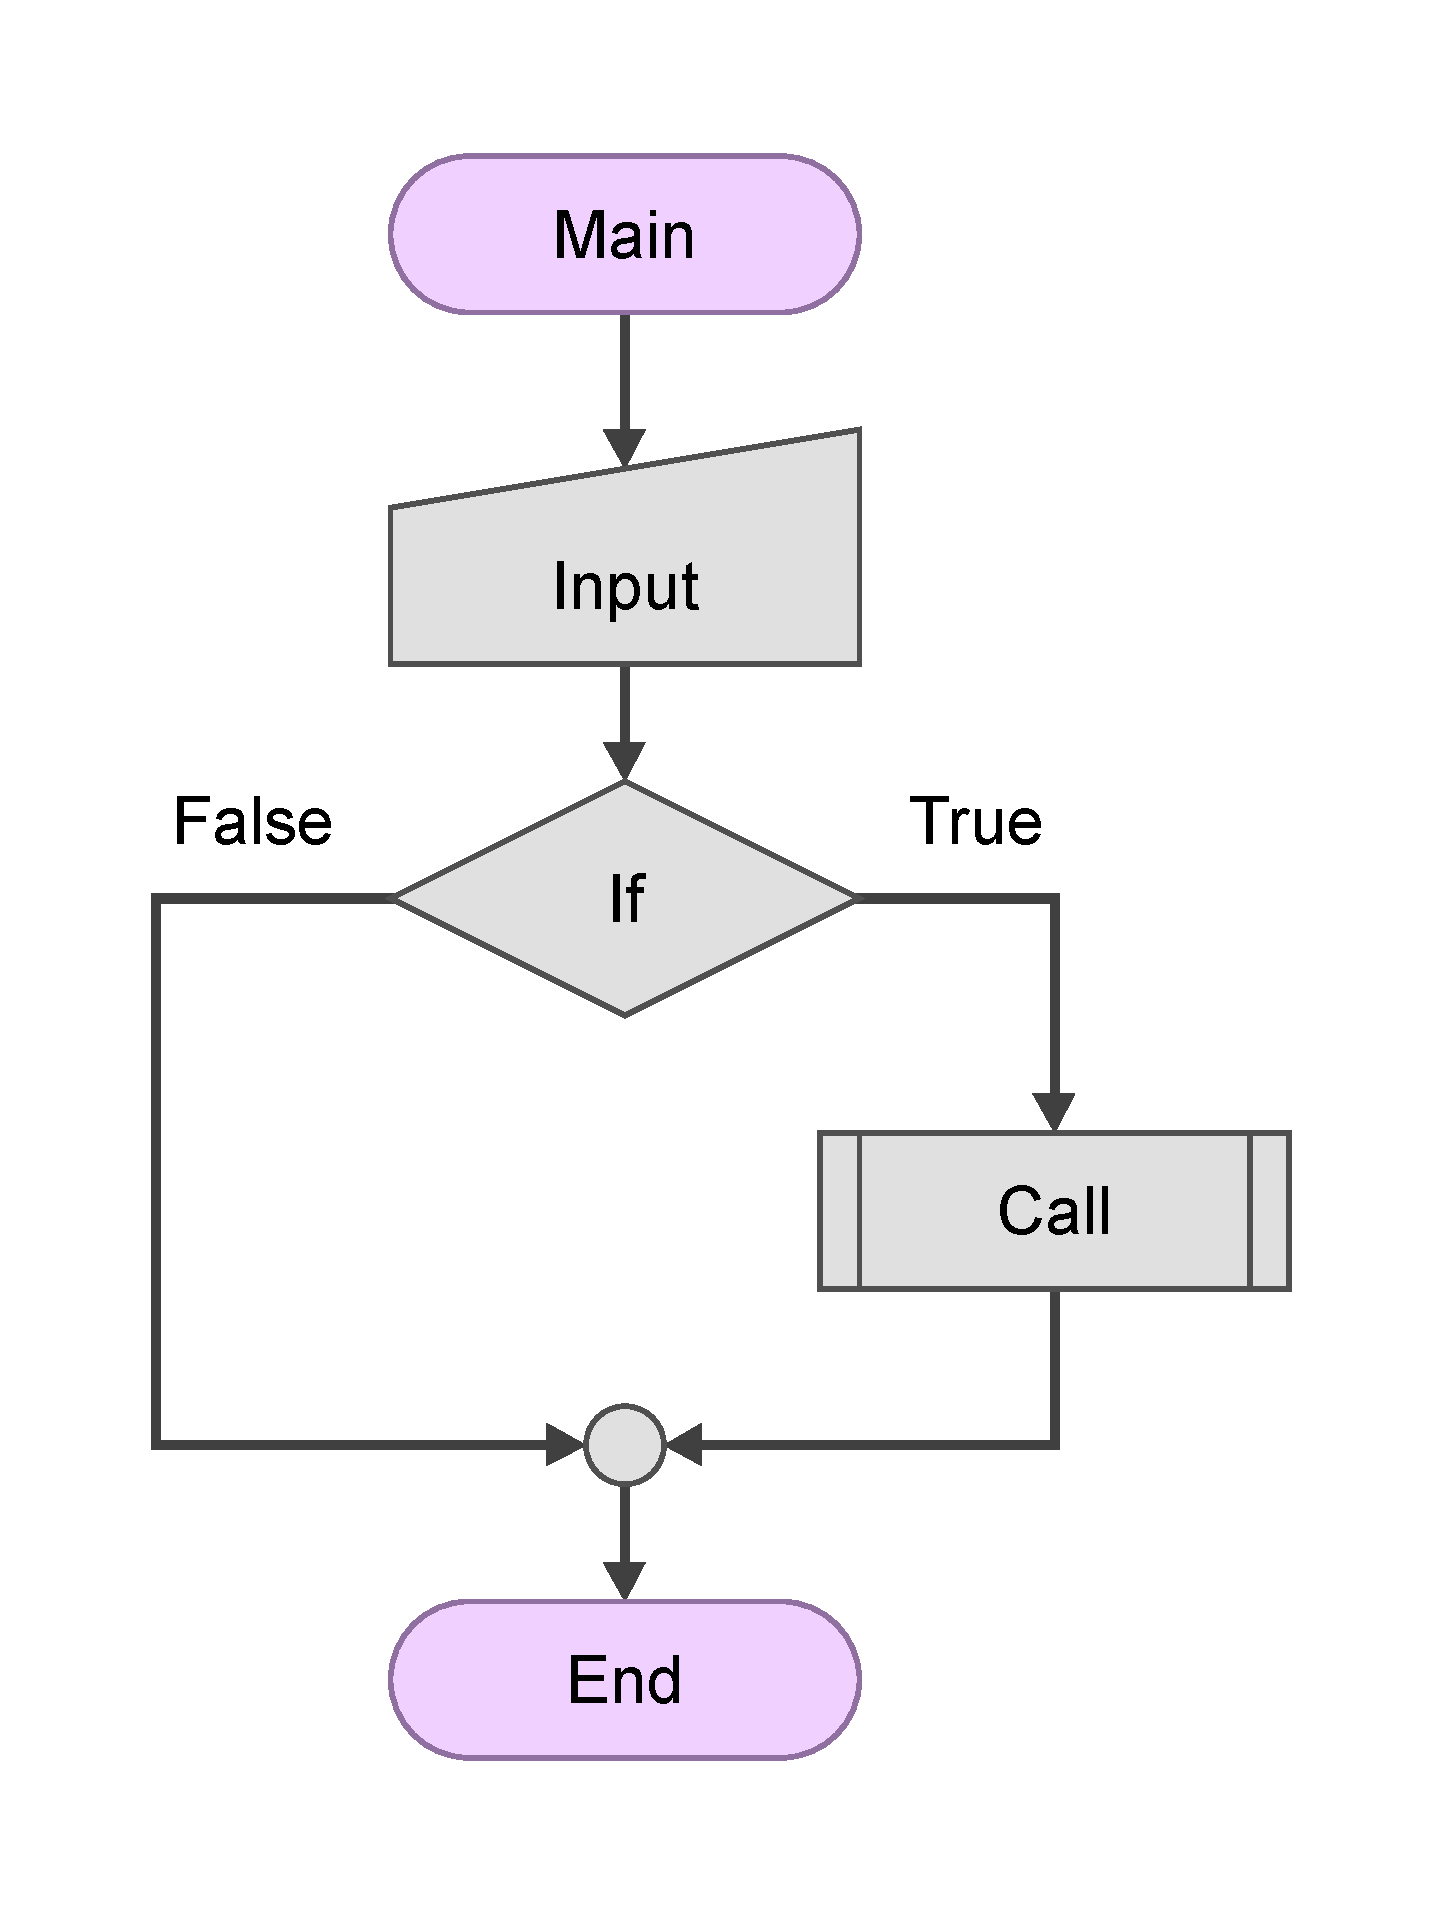
\includegraphics[scale=0.3]{figures/chart.pdf}
    \caption{Example figure in \LaTeX.}
    \label{fig:chart_a}
\end{figure}

\clearpage %  use command \clearpage when you want section or text to appear in the next page.

\section{Example of an algorithm in \LaTeX}
Algorithm~\ref{algo:algo_example} is a good example of an algorithm in \LaTeX.  
\begin{algorithm}
    \caption{Example caption: sum of all even numbers}
    \label{algo:algo_example}
    \begin{algorithmic}[1]
        \Require{$ \mathbf{x}  = x_1, x_2, \ldots, x_N$}
        \Ensure{$EvenSum$ (Sum of even numbers in $ \mathbf{x} $)}
        \Statex
        \Function{EvenSummation}{$\mathbf{x}$}
        \State {$EvenSum$ $\gets$ {$0$}}
        \State {$N$ $\gets$ {$length(\mathbf{x})$}}
        \For{$i \gets 1$ to $N$}                    
        \If{$ x_i\mod 2 == 0$}  \Comment check if a number is even?
        \State {$EvenSum$ $\gets$ {$EvenSum + x_i$}}
        \EndIf
        \EndFor
        \State \Return {$EvenSum$}
        \EndFunction
    \end{algorithmic}
\end{algorithm}
 
\section{Example of code snippet  in \LaTeX}

Code Listing~\ref{list:python_code_ex} is a good example of including a code snippet in a report. While using code snippets, take care of the following:
\begin{itemize}
    \item do not paste your entire code (implementation) or everything you have coded. Add code snippets only. 
    \item The algorithm shown in Algorithm~\ref{algo:algo_example} is usually preferred over code snippets in a technical/scientific report. 
    \item Make sure the entire code snippet or algorithm stays on a single page and does not overflow to another page(s).  
\end{itemize}

Here are three examples of code snippets for three different languages (Python, Java, and CPP) illustrated in Listings~\ref{list:python_code_ex}, \ref{list:java_code_ex}, and \ref{list:cpp_code_ex} respectively.  

\begin{lstlisting}[language=Python, caption={Code snippet in \LaTeX ~and  this is a Python code example}, label=list:python_code_ex]
import numpy as np

x  = [0, 1, 2, 3, 4, 5] # assign values to an array
evenSum = evenSummation(x) # call a function

def evenSummation(x):
    evenSum = 0
    n = len(x)
    for i in range(n):
        if np.mod(x[i],2) == 0: # check if a number is even?
            evenSum = evenSum + x[i]
    return evenSum
\end{lstlisting}

Here we used  the ``\textbackslash clearpage'' command and forced-out the second listing example onto the next page. 
\clearpage  %
\begin{lstlisting}[language=Java, caption={Code snippet in \LaTeX ~and  this is a Java code example}, label=list:java_code_ex]
public class EvenSum{ 
    public static int evenSummation(int[] x){
        int evenSum = 0;
        int n = x.length;
        for(int i = 0; i < n; i++){
            if(x[i]%2 == 0){ // check if a number is even?
                evenSum = evenSum + x[i];
            }
        }
        return evenSum;     
    }
    public static void main(String[] args){ 
        int[] x  = {0, 1, 2, 3, 4, 5}; // assign values to an array
        int evenSum = evenSummation(x);
        System.out.println(evenSum);
    } 
} 
\end{lstlisting}


\begin{lstlisting}[language=C, caption={Code snippet in \LaTeX ~and  this is a C/C++ code example}, label=list:cpp_code_ex]
int evenSummation(int x[]){
    int evenSum = 0;
    int n = sizeof(x);
    for(int i = 0; i < n; i++){
        if(x[i]%2 == 0){ // check if a number is even?
            evenSum = evenSum + x[i];
    	}
    }
    return evenSum;     
}

int main(){
    int x[]  = {0, 1, 2, 3, 4, 5}; // assign values to an array
    int evenSum = evenSummation(x);
    cout<<evenSum;
    return 0;
}
\end{lstlisting}



\section{Example of in-text citation style}
\subsection{Example of the equations and illustrations placement and reference in the text}
Make sure whenever you refer to the equations, tables, figures, algorithms,  and listings for the first time, they also appear (placed) somewhere on the same page or in the following page(s). Always make sure to refer to the equations, tables and figures used in the report. Do not leave them without an \textbf{in-text citation}. You can refer to equations, tables and figures more them once.

\subsection{Example of the equations and illustrations style}
Write \textbf{Eq.} with an uppercase ``Eq`` for an equation before using an equation number with (\textbackslash eqref\{.\}). Use ``Table'' to refer to a table, ``Figure'' to refer to a figure, ``Algorithm'' to refer to an algorithm and ``Listing'' to refer to listings (code snippets). Note that, we do not use the articles ``a,'' ``an,'' and ``the'' before the words Eq., Figure, Table, and Listing, but you may use an article for referring the words figure, table, etc. in general.

For example, the sentence ``A report structure is shown in \textbf{the} Table~\ref{tab:gen_template}'' should be written as ``A report structure is shown \textbf{in} Table~\ref{tab:gen_template}.'' 
 

\section{Summary}
Write a summary of this chapter.

~\\[5em]
\noindent
{\huge\textbf{Note:}} In the case of \textbf{software engineering} project a Chapter ``\textbf{Testing and Validation}'' should precede the ``Results'' chapter. See Section~\ref{subsec:se_chpters} for report organization of such project. 


\chapter{System Study, Analysis and Design}

\section{Overview of the System}



\chapter{Presentation of Results}

\section{Introduction}
This chapter shows screenshots of the system interfaces and also explains the programming environment, .......................
\chapter{Limitations, Recommendations and Conclusion}

\section{Introduction}
This chapter presents a conclusion to the project, .............. 
\newpage


%create references professionally, this is a demo
\textbf{References}

\newpage
This template was developed using \LaTeX{}


\bibliographystyle{plain}
\bibliography{References}

\end{document}
